\indent Para verificar el correcto funcionamiento de nuestro algoritmo , elaboramos disversos tests,
los cuales ser\'an enunciados a continuaci\'on.\\

\begin{center}
 \textbf{No existe arbol que conecte todas las salas}
\end{center}

Este caso se da cuando en cualquier camino nos encontramos con paredes irrompibles sin la posibilidad de esquivarlas\\

 Para este tipo de testeo mostraremos a continuaci\'on un ejemplo del mismo, exponiendo su respectivo resultado. Adem\'as veremos m\'as adelante, que por el desarrollo de nuestro algoritmo y sus respectivas podas este ser\'a el peor caso en referencia a la perfomance del mismo.\\
 
 Con un:
 
\vspace*{0.3cm} \vspace*{0.3cm}
  \begin{center}
 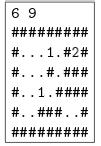
\includegraphics[scale=0.65]{./EJ2/ej2sinsolucion.jpeg}
\\{$Ejemplo$ \ 2.1.1 - $Caso$ $Sin$ $Soluci$\'on}
  \end{center}
  \vspace*{0.3cm}

El grafo que representa a este tipo es de la siguiente forma:\\

\vspace*{0.3cm} \vspace*{0.3cm}
  \begin{center}
 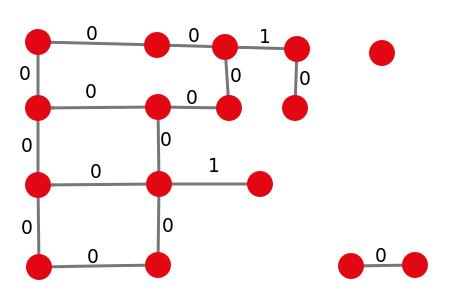
\includegraphics[scale=0.5]{./EJ2/ej2grafosinsolucion.jpeg}
 \\{$Ejemplo$ \ 2.1.2 - $Caso$ $Sin$ $Soluci$\'on}
  \end{center}
  \vspace*{0.3cm}

  Obtuvimos el siguiente resultado:

$Esfuerzo$ $total: $ $-1$\\




 \begin{center}
 \textbf{Existe un camino que conecta todas las salas de esfuerzo 0}
\end{center}

Esta versi\'on se da cuando la suma de los pesos de las aristas del AGM obtenido es 0. 

Para este tipo de testeo mostraremos a continuaci\'on un ejemplo del mismo, exponiendo su respectivo resultado.\\

 
 Con un:
 
\vspace*{0.3cm} \vspace*{0.3cm}
  \begin{center}
 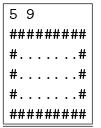
\includegraphics[scale=0.65]{./EJ2/ej2sinpared.jpeg}
 \\{$Ejemplo$ \ 2.2.1 - $Caso$ $Sin$ $Romper$ $Paredes$}
  \end{center}
  \vspace*{0.3cm}

El grafo que representa a este tipo es de la siguiente forma:\\

\vspace*{0.3cm} \vspace*{0.3cm}
  \begin{center}
 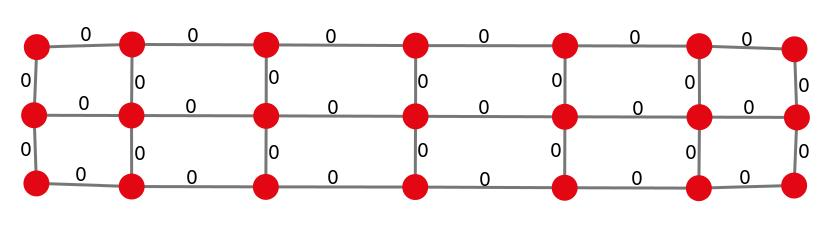
\includegraphics[scale=0.5]{./EJ2/ej2grafosinpared.jpeg}
 \\{$Ejemplo$ \ 2.2.2 - $Caso$ $Sin$ $Romper$ $Paredes$}
  \end{center}
  \vspace*{0.3cm}

  Obtuvimos el siguiente resultado:

$Esfuerzo$ $total: $ $0$


\begin{center}
 \textbf{El AGM es todo el grafo}
\end{center}

Este caso se da cuando el laberinto no presenta varios caminos para poder ir a las salas sino un \'unico camino 


Aqu\'i veremos, un ejemplo del conjunto de test de este tipo, exponiendo su respectivo resultado.\\
 
 Con un:
 
\vspace*{0.3cm} \vspace*{0.3cm}
  \begin{center}
 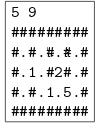
\includegraphics[scale=0.65]{./EJ2/ej2completo.jpeg}
\\ {$Ejemplo$ \ 2.3.1 - $Caso$ $AGM = GRAFO$}
  \end{center}
  \vspace*{0.3cm}

El grafo que representa a este tipo es de la siguiente forma:\\

\vspace*{0.3cm} \vspace*{0.3cm}
  \begin{center}
 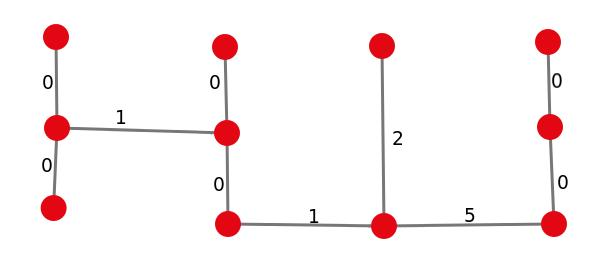
\includegraphics[scale=0.5]{./EJ2/ej2grafocompleto.jpeg}
 \\{$Ejemplo$ \ 2.3.2 - $Caso$ $AGM = GRAFO$}
  \end{center}
  \vspace*{0.3cm}

  Obtuvimos el siguiente resultado:

$Esfuerzo$ $total: $ $9$


\begin{center}
 \textbf{Camino por las salas random}
\end{center}

Este caso se da cuando hay posiblidad de conectar todas las salas rompiendo una cierta cantidad de paredes, tambi\'en denominado caso random debido al desarrollo de nuestro algoritmo.\\

Siguiendo el desarrollo de dicho informe a continuaci\'on mostraremos, un ejemplo del grupo de test de este estilo, exponiendo su respectivo resultado.\\
 
 Con un:
 
\vspace*{0.3cm} \vspace*{0.3cm}
  \begin{center}
 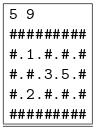
\includegraphics[scale=0.65]{./EJ2/ej2random.jpeg}
\\ {$Ejemplo$ \ 2.4.1 - $Caso$ $Random$}
  \end{center}
  \vspace*{0.3cm}

El grafo que representa a este tipo es de la siguiente forma:\\

\vspace*{0.3cm} \vspace*{0.3cm}
  \begin{center}
 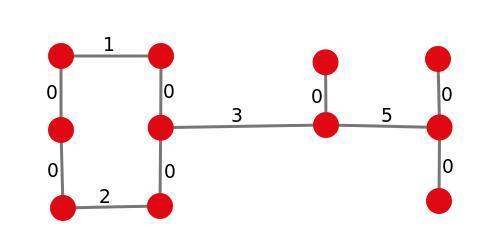
\includegraphics[scale=0.5]{./EJ2/ej2graforandom.jpeg}
 \\{$Ejemplo$ \ 2.4.2 - $Caso$ $Random$}
  \end{center}
  \vspace*{0.3cm}

  Obtuvimos el siguiente resultado:

$Esfuerzo$ $total: $ $9$\\


\textbf{Aclaraciones:} 
\begin{itemize}
\item Nodo aislado significa que esta rodeado de paredes irrompibles no hay camino posible de conectar dicho nodo a la componente conexa.
\end{itemize}